\section{Background and Overview}
\label{sec:layeredbsdf:background}

In this section, we explicitly state the assumptions of our method, provide background on the standard path formulation of light transport, and provide a quick overview of the rest of the chapter.

\subsection{Assumptions}
Although light generally enters and leaves the layer from different locations, we note that when the layers are thin and the lighting is comparably distant, the entrance and departure locations will be close enough to each other. We assume it is acceptable to ignore this displacement, allowing us to describe the light transport in the layers using BSDFs, rather than BSSRDFs (Figure~\ref{fig:layeredbsdf:assumption}).

\begin{figure}[h]
	\centering
	
\includegraphics[width=0.5\textwidth]{layeredbsdf/illustration/assumption.pdf}
	\caption[Small displacement assumption]{\label{fig:layeredbsdf:assumption}
		\textbf{Small displacement assumption:}
		when light hits a thin layer, it gets reflected and refracted by the interfaces and scattered and absorbed internally.
		Since the geometric thickness $h$ of the layer is small, we assume the displacements (e.g., $\Delta x$) of light's entrance and departure locations can be neglected.
	}
\end{figure}

Furthermore, we assume that the spatial variation of layer properties is slow enough that a BSDF evaluation at a single surface point can locally approximate them as spatially uniform. This is related to the above in assuming that the horizontal spreading of light is small enough to be negligible.

In fact, these are the \emph{only} approximating assumptions of our approach, which otherwise offers unbiased accuracy and full flexibility in setting the layer properties and varying them spatially.

\subsection{Review of Veach's path integral formulation}
\label{subsec:path_int}

In the Veach formulation of light transport \cite{veach1997robust}, light paths are defined as sequences of vertices connected by segments.
The value of a light transport integral (for example, but not necessarily limited to, a pixel value) is written as
\begin{equation}
	I = \int_\Omega f(\bar x) \intd \mu(\bar x),
\end{equation}

where $\bar x = (x_0, \dots, x_k)$ is a path with $k$ segments and $k + 1$ vertices on the surfaces or within the participating media of a scene.
$\Omega$ is the space of all paths and is defined as the union of $\Omega_k$ for $k \geq 0$, where $\Omega_k$ indicates the set of paths of length $k$.
Furthermore, $f(\bar x)$ is the path contribution to the integral, and $\mu(\bar x)$ is a special measure on the path space, defined as the product of area measures on the vertices $x_i$. The contribution $f(\bar x)$ is a product of vertex terms (normally BSDFs and phase functions) and geometry terms corresponding to path segments. The geometry terms contain the squared distance between the two vertices in the denominator; this is a significant source of variance when trying to connect independently sampled vertices on thin layer configurations.

\subsection{Overview}

In Section \ref{sec:layeredbsdf:pathformulation}, we describe our path formulation of layered light transport. Our path integral differs from Veach's formulation in that it is \emph{position-free}. The key idea is that on an infinite flat slab, the horizontal positions of vertices do not matter: it is only the vertical position (depth) of a vertex, and the \emph{directions} between vertices, that are relevant to a light transport integral. The vertices are defined by their depth in the layer, as opposed to a full 3D position, and the segments have variable unit directions.

It is important to note that our position-free formulation is not just a simplified specialization of the standard formulation to the flat slab setting, but in fact a new approach that achieves much superior variance to the standard formulation. The key benefit of this new formulation is that it does not contain the inverse square distance falloff terms that are required between any two vertices with full positional information. The leads to high variance, even in advanced estimators such as bidirectional and Metropolis transport, which in fact perform even worse in this setting than unidirectional; see Figure \ref{fig:layeredbsdf:equal_time_compare} for examples.

In contrast, our approach leads to an efficient estimator based on unidirectional sampling with next event estimation, and an even more efficient bidirectional estimator. The unidirectional performs similarly (though usually not better) in simpler cases, but in challenging cases with sharp and/or anisotropic BSDFs and phase functions, the bidirectional version is clearly more efficient (Figure~\ref{fig:layeredbsdf:equal_time_compare}, bottom). 
Figure \ref{fig:layeredbsdf:lobes} demonstrates the performance of the estimators through BSDF lobe visualization, also showing a close match to ground truth. In Section \ref{sec:layeredbsdf:ours}, we describe these two estimators in detail, and also focus on the two additional operations critical for integrating a BSDF into a practical renderer: importance sampling and pdf evaluation.

\begin{figure}[h]
	\centering
	\setlength{\resLen}{1.4in}
	\addtolength{\tabcolsep}{0pt}
	\begin{tabular}{ccc}
		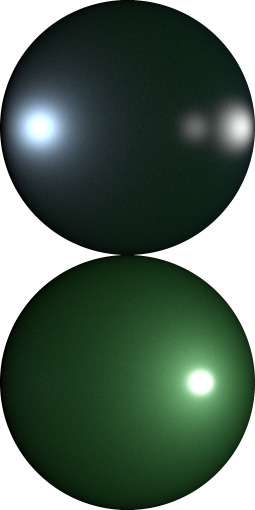
\includegraphics[width=\resLen]{layeredbsdf/validations/lobe_bsdf/bsdf_sample_all.jpg} &
		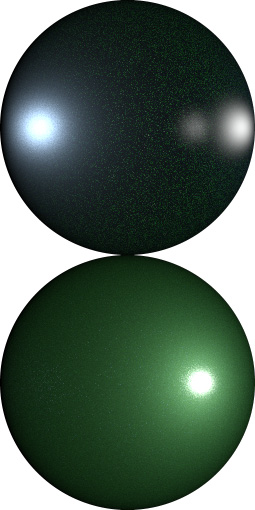
\includegraphics[width=\resLen]{layeredbsdf/validations/lobe_bsdf/bsdf_eval_uni_all.jpg} &
		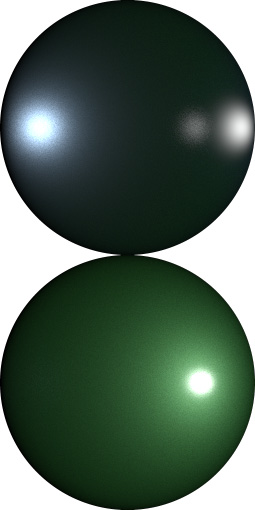
\includegraphics[width=\resLen]{layeredbsdf/validations/lobe_bsdf/bsdf_eval_bi_all.jpg} \\
		Ground truth &
		Our unidir. &
		Our bidir. \\
	\end{tabular}
	\caption[Outgoing lobes of a layered BSDF]{\label{fig:layeredbsdf:lobes}
		\textbf{Outgoing lobes of a layered BSDF} (reflection and transmission) visualized as projected hemispheres. \textbf{Left:} ground truth computed by sampling and binning the light paths. \textbf{Middle:} Our unidirectional estimator. \textbf{Right:} Our bidirectional estimator (same time).
	}
\end{figure}

Finally, we present results in Section \ref{sec:layeredbsdf:results}, and summarize in Section \ref{sec:layeredbsdf:conclusion}.

% \subsection{Applying a Monte Carlo estimator}
% \label{sec:applymc}
%
% To evaluate the BSDF value $f_l(\omegain, \omegaout)$ for given query directions $\omegain$ and $\omegaout$, we need to evaluate the path integral of Eq.~\eqref{eq:pathintegral} by sampling paths $\bar x$ from some distribution, and weighting the paths by their contribution, divided by their probability densities in the measure $\mu(\bar x)$, i.e. the product of solid angle measures at the internal directions of the path.
%
% Consider the specific example of $\Omega_3(\omegain, \omegaout)$, i.e. the subspace of paths with three vertices, corresponding to a transmit-reflect-transmit (TRT) configuration.
% For paths in this subspace, only the directions $\bd_1$ and $\bd_2$ are ``free parameters'' participating in the integration, and the measure is simply the product of solid angle measures at $\bd_1$ and $\bd_2$.
% This suggests a simple and effective approach for choosing $\bd_1$ and $\bd_2$ (and thus $\bar x$): to importance-sample the top interface BSDF $f_\uparrow$ twice, by using $\omegain$ and $\omegaout$ as the incoming directions, respectively (Figure~\ref{fig:mis_local}-a).
% Alternatively, one can sample $\bd_1$ and $\bd_2$ by first drawing $\bd_1$ using $f_\uparrow$ (given $\omegain$) and then $\bd_2$ (given $\bd_1$) using $f_\downarrow$ (Figure~\ref{fig:mis_local}-b).
% This method is more efficient when the bottom interface is close to specular.
% Both strategies can be combined using MIS to provide a robust sampling scheme for light transport paths $\bar{x} \in \Omega_3(\omegain, \omegaout)$.
%
% In standard rendering systems, a BSDF sampling procedure commonly returns a ``weight'', defined as the BSDF value in the sampled direction $\bom$, times the cosine term, divided by the probability density (pdf) of picking the direction in the solid angle measure.
% %\szrem{Need a figure to make this part clearer.}
% This makes it particularly convenient to compute the path contribution divided by the pdf: simply multiply the two weights returned by importance-sampling $\bd_1$ and $\bd_2$, additionally multiplied by the BSDF at the bottom interface, $f_s(x_2, \bd_1, -\bd_2)$.
%
% Furthermore, it is clear that there is nothing specific about the TRT mode here, and a minor modification of this approach works for camera and light subpaths of any length. In our concrete implementation, the light subpath has up to one vertex, while the camera subpath can have any length.
